\documentclass[border=10pt]{standalone}
\usepackage{tikz}
\begin{document}
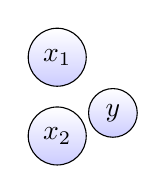
\begin{tikzpicture}[sibling distance=10em,
  every node/.style = {shape=circle, rounded corners,
    draw, align=center,
    top color=white, bottom color=blue!20}]]

    \node(a) {$x_1$};
    \node(b) [below of=a] {$x_2$};
    \node(y) [below right of=a] {$y$};

\end{tikzpicture}
\end{document}

% \documentclass[12pt,letterpaper]{report}
% \usepackage{pgf, tikz}
% \usetikzlibrary{arrows, automata}

% \begin{document}

%     \begin{tikzpicture}[
%             > = stealth, % arrow head style
%             shorten > = 1pt, % don't touch arrow head to node
%             auto,
%             node distance = 3cm, % distance between nodes
%             semithick % line style
%         ]

%         \tikzstyle{every state}=[
%             draw = black,
%             thick,
%             fill = white,
%             minimum size = 4mm
%         ]

%         \node[state] ($a$) {$s$};
%         \node[state] (v1) [above right of=s] {$v_1$};
%         \node[state] (v2) [right of=s] {$v_2$};
%         \node[state] (v3) [below right of=s] {$v_2$};
%         \node[state] (t) [right of=v2] {$t$};

%         \path[->] (s) edge node {18} (v1);
%         \path[->] (s) edge node {1} (v2);
%         \path[->] (s) edge node {1} (v3);
%         \path[->] (v2) edge node {2} (v1);
%         \path[->] (v3) edge node {1} (v2);
%         \path[->] (v1) edge node {20} (t);

%         \draw[red, dashed] (1, 2) -- (1, -2);
%     \end{tikzpicture}

% \end{document}